% which is a fork of the unofficial University of Texas at Arlington Math Poster template:
% which is a fork of the unofficial University of Lethbridge Poster template: https://www.overleaf.com/latex/templates/university-of-lethbridge-unofficial-poster-template/nddfzgvqvfwf
% which is a fork of unofficial University of Alberta Poster template: 
% which is a fork of Yale template: https://www.overleaf.com/latex/templates/yale-poster-template/rjpgqfgvsjcv
% which is a fork of the UMich template https://www.overleaf.com/latex/templates/university-of-michigan-umich-poster-template/xpnqzzxwbjzc
% which is fork of the MSU template https://www.overleaf.com/latex/templates/an-unofficial-poster-template-for-michigan-state-university/wnymbgpxnnwd
% which is a fork of https://www.overleaf.com/latex/templates/an-unofficial-poster-template-for-new-york-university/krgqtqmzdqhg
% which is a fork of https://github.com/anishathalye/gemini
% also refer to https://github.com/k4rtik/uchicago-poster
% and https://www.overleaf.com/latex/templates/tcd-poster-template/gtnrnpdmqxgk

\documentclass[final]{beamer}

% ====================
% Packages
% ====================

\usepackage[T1]{fontenc}
\usepackage[utf8]{luainputenc}
\usepackage{lmodern}
\usepackage[size=custom, width=122,height= 91, scale=1.2]{beamerposter} %OG size=custom, width=122,height=91, scale=1.2
\usetheme{gemini}
\usecolortheme{msu}
\usepackage{graphicx}
\usepackage{booktabs}
\usepackage{tikz}
\usepackage{pgfplots}
\pgfplotsset{compat=1.14}
\usepackage{anyfontsize}

% ====================
% Lengths
% ====================

% If you have N columns, choose \sepwidth and \colwidth such that
% (N+1)*\sepwidth + N*\colwidth = \paperwidth
\newlength{\sepwidth}
\newlength{\colwidth}
\setlength{\sepwidth}{0.025\paperwidth}
\setlength{\colwidth}{0.3\paperwidth}

\newcommand{\separatorcolumn}{\begin{column}{\sepwidth}\end{column}}

% ====================
% Title
% ====================

\title{Gödel's First Incompleteness Theorem}

\author{Bruno Cassani}
% add following line if you have co-author(s)
% Coauthor One$^{2}$, Coauthor Two$^{3}$

\institute[shortinst]{\textbf{Morrissey College of Arts and Sciences}, Boston College}

% ====================
% Footer (optional)
% ====================

\footercontent{  \hfill
  \href{mailto:cassanib@bc.edu}{cassanib@bc.edu}}
% (can be left out to remove footer)

% ====================
% Logo
% ====================

% use this to include logos on the left and/or right side of the header:
% Left: institution
 \logoright{
\includegraphics[height=8cm]{logos/bclogo.png}}
% Right: funding agencies and other affilations 
%\logoright{\includegraphics[height=7cm]{logos/NSF.eps}}

% ====================
% Body. Real Poster starts here
% ====================

\begin{document}



\begin{frame}[t]
\begin{columns}[t]
\separatorcolumn

\begin{column}{\colwidth}



  \begin{alertblock}{Theorem}

    To every $\omega$-consistent recursive class $\small{K}$ of formulae there correspond recursive class-signs $r$, such that neither $vGen(r)$ nor $\neg vGen(r)$ belongs to $Flg(k)$.

    \begin{figure}
      \centering
            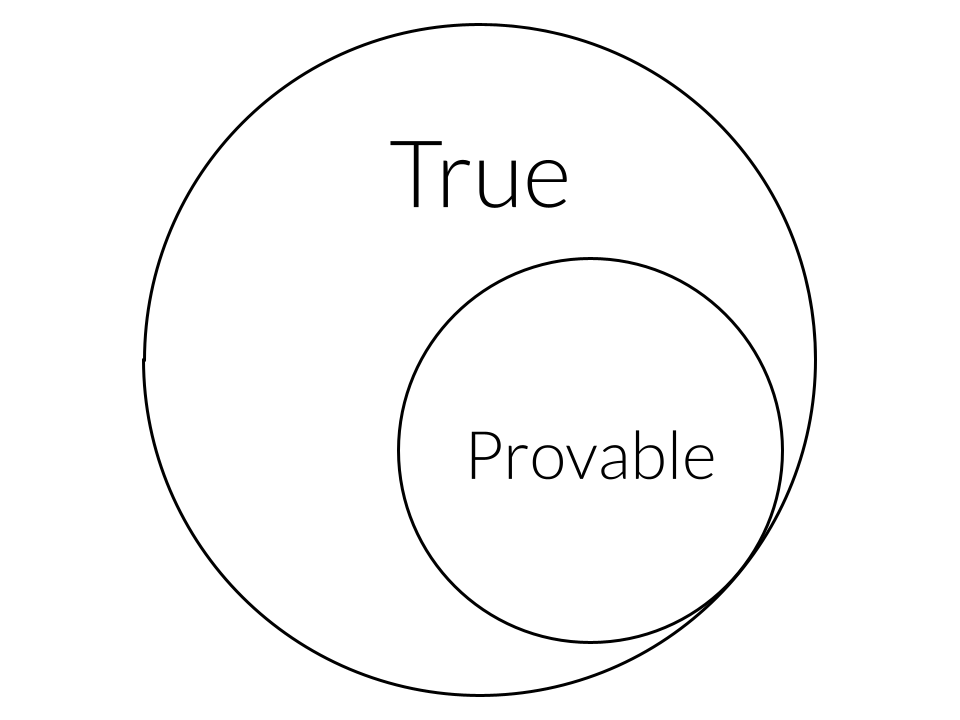
\includegraphics[width=0.5\textwidth]{figures/Draw_1.png}
    \end{figure}

    In other words, every reasonable recursive axiomatic proposition of number theory will always have propositions that cannot be proven nor disproven.
    
  \end{alertblock}
  
\begin{block}{Background}

    \begin{itemize}
      \item Before Gödel, metamathematicians expected math to eventually be \textbf{complete}, i.e., to be able to prove everything given the right amount of axioms.
      \item In the early 20th century, set theory paradoxes like those proposed by Bertrand Russell raised questions about the \textbf{consistency} of math.
      \item Gödel was trying to solve Hilbert's Second problem — he wanted to know if math had any inherent contradictions and if truth was self-evident.
        
    \end{itemize}

\end{block}

\begin{exampleblock}{Proposition}

      Statements \textit{of} number theory could also be \textit{about} number theory.

\end{exampleblock}

\begin{block}{Gödel Numbering}

      To investigate the proposition, Gödel needed math to be self-referential. He created his own $Encode(G)$ function to turn mathematical statements into unique natural numbers. To do so, he would first need to convert each mathematical symbol into a number. Thus, he created a numbering system where each symbol has its own unique natural number to be used for encoding.

    \begin{table}[h]
    \centering
    \begin{tabular}{c|c}
    \textbf{Constant Sign} & \textbf{Gödel Number} \\ \hline
    $\neg$ & 1 \\ 
    $\lor$ & 2 \\ 
    $\supset$ & 3 \\ 
    $\exists$ & 4 \\ 
    $=$ & 5 \\ 
    $\vdots$ & $\vdots$ \\ 
    \end{tabular}
    \end{table}

    In theory, the symbols have no meaning, the axioms and formulas constructed from them are what give them their meaning.
    
  \end{block}

\end{column}

\separatorcolumn %NEW COLUMN%

\begin{column}{\colwidth}

  \begin{block}{Encoding}

    Given a sequence of Gödel numbers $(x_1, x_2, \dots, x_n)$, the encoding is the product of the first $n$ prime numbers raised to the values in the sequence.

    $$Encode(x_1, x_2, \dots, x_n) = 2^{x_1} \times 3^{x_2} \times \ldots \times p_n^{x_n}$$

    This way, any given mathematical expression can be encoded algebraically. Besides, the statements can be decoded through prime factorization.

    Note: $Encode(A)$ is often written as $\ulcorner \!A \urcorner$.

  \end{block}

 \begin{block}{Provability}

Since statement $A$ can be proved through an axiom $B$, and $\ulcorner \!A \urcorner)$ and $\ulcorner \!B \urcorner$ are unique numbers, Gödel proposed that there must be a mathematical relation between the two.

 \begin{itemize}
    
    \item We can express this relation as a function $Provability(\ulcorner \!A \urcorner)$ that determines whether a statement $A$ is provable within the formal system.
    
    \item This function is essentially a binary predicate that determines if $A$ can be proved with the current axioms.
    
    \end{itemize}

 \end{block}


 \begin{block}{Self-reference by diagonalization}

    Enumerate all formulas in the formal system $F$ with exactly one free variable:
    
    \[
    \begin{array}{c|c|c|c|c}
    & n=1 & n=2 & \cdots & n = j \\
    \hline
    F_1(n) & F_1(1) & F_1(2) & \cdots & F_1(j) \\
    F_2(n) & F_2(1) & F_2(2) & \cdots & F_2(j) \\
    \vdots & \vdots & \vdots & \ddots & \vdots \\
    F_j(n) & F_j(1) & F_j(2) & \cdots & F_j(j) \\
    \end{array}
    \]


Each entry represents a formula \( F_i(n) \), where \( i \) represents the formula number and \( n \) represents the parameter.
\end{block}

\begin{block}{Gödel Statement}

Construct a new formula $G$, asserting the negation of provability for each formula $F_j(j)$ in the table. This is what is known as the Gödel statement:
$$G \equiv \neg Provability(F_j(j))$$

 Now, consider the truth value of $G$. If $G$ were false, then by its own definition, each $F_j(j)$ would be provable and thus true. But the definition of $G$ implies the opposite; since math is consistent, $G$ must be true. Since $G$ cannot be consistently proven or disproven within the system, it follows that $G$ is true but unprovable within $F$.
 
 \end{block}

\end{column}


%%THIRD COLUMN
\separatorcolumn

\begin{column}{\colwidth}

\begin{block}{Axiomatization}
Although the proof works, one might argue that the Gödel statement could be made into an axiom to trivialize the problem.\\
However, doing so would only create a new system where the current $G$ could be proved; it would change the nature of the new system, leading to further contradictions.

\end{block}

\begin{block}{Implications}

 \begin{itemize}
      \item Mathematics
        \begin{itemize}
        
            \item Forced meta-mathematics past Russell's \textit{Principia Mathematica}.
            \item Established a mutual exclusivity between consistency and completeness of recursive formal systems.
            \item No single formal system can capture all mathematical truths, showing the inherent incompleteness of axiomatic systems of logic.
            
        \end{itemize}
      
      \item Computer Science
        \begin{itemize}

            \item Popularized the arithmetization of syntax in the years leading up to the first computers.
            \item Inspired Turing, and by consequence the field of computability theory.
            \item Furthered the complexity of the discussions on the limitations of computers and artificial intelligence.
            
        \end{itemize}
      
      \item Philosophy
        \begin{itemize}
            \item Directly challenges the idea of determinism and a fully knowable universe.
            \item Furthers debate on the nature of knowledge and the transcendence of human intuition.
        \end{itemize}
        
    \end{itemize}
    
\end{block}

  \begin{block}{References}
    \nocite{*}
    \footnotesize{\bibliographystyle{plain}\bibliography{poster}}

  \end{block}

\end{column}

\separatorcolumn
\end{columns}
\end{frame}

\end{document}
